\documentclass[hyperref=unicode, aspectratio=169]{beamer}
\usepackage[utf8]{inputenc}
\usepackage[T2A]{fontenc}
\usepackage[russian]{babel}
\usepackage{csquotes}
\usepackage{tikzit}
\usepackage[justification=centering]{caption}
\usepackage{mathabx}
\usepackage{bookmark}
\usepackage{makecell}
\usepackage{listings}
\usepackage{flowchart}
\usepackage{subcaption}
\usepackage{caption}

\captionsetup[figure]{labelformat=empty}


\title[]{Жадные алгоритмы для построения многопроцессорного списочного расписания}
\usetheme{Madrid}
\author[]{Савицкий Илья\\Научный руководитель: к.т.н. доцент Костенко Валерий Алексеевич}
% \medskip
% \texttt{Научный руководитель: к.т.н. доцент Костенко Валерий Алексеевич}
\date{27 апреля 2023 г.}
\logo{
\includegraphics[width=1.5cm]{imgs/asvk-logo.png}}


\definecolor{ASVKaccent}{rgb}{0.20392,0.02745,0.34509}
\usecolortheme[named=ASVKaccent]{structure}

\input{block-schemas.tikzstyles}

\begin{document}

\begin{frame}
    \titlepage
\end{frame}

\section{Цель и задачи дипломной работы}
\begin{frame}
    \frametitle{Цели и задачи ВКР}
    Целью ВКР является разработка детерминированного алгоритма построения многопроцессорного расписания с дополнительными ограничениями.

    Для достижения указанной цели требуется:
    \begin{enumerate}
        \item Провести аналитический обзор алгоритмов построения списочных расписаний с целью выявления алгоритмов, которые возможно модифицировать под поставленную задачу и имеют хорошую возможность масштабирования.
        \item Разработать и реализовать алгоритмы.
        \item Провести исследование качества решений и временной сложности алгоритмов.
    \end{enumerate}
\end{frame}

\section{Описание прикладной задачи}
\begin{frame}
    \frametitle{Постановка задачи}
    \begin{columns}
        \begin{column}{0.60\textwidth}
            \begin{enumerate}
                \item Ориентированный граф работ $G$ без циклов, в котором дуги - зависимости по данным, а вершины - задания. Вершин $n$, дуг $m$
                \item Вычислительная система, состоящая из $p$ различных процессоров.
                \item Матрица $C_{ij}$ длительности выполнения работ на процессорах, $i=1 \dots n, j=1 \dots p$. Каждая строка этой матрицы - длины выполнения $n$-й задачи на $p$ процессорах. 
                \item Матрица $D_{kl}$ передач данных между процессорами, $k=1 \dots p, l = 1 \dots p, D_{kk} = 0$. $D_{ij}$-й элемент этой матрицы - время передачи данных между процессорами $i$ и $j$.
            \end{enumerate}
        \end{column}
        \begin{column}{0.40\textwidth}
            \begin{figure}
                \ctikzfig{graph_schema}
                \captionsetup{labelformat=empty}
                \caption{Граф потока данных}
            \end{figure}
        \end{column}
    \end{columns}
\end{frame}

\begin{frame}
    \frametitle{Расписание}
    Расписание программы определено, если определены
    \begin{enumerate}
        \item Множества процессоров и работ
        \item Привязка
        \item Порядок
    \end{enumerate}
    \par
    \textbf{Привязка} - всюду определенная на множестве работ функция, которая задает распределение работ по процессорам.
    \par
    \textbf{Порядок} задает ограничения на последовательность выполнения работ и является отношением частичного порядка, удовлетворяющим условиям ацикличности и транзитивности. Отношение порядка на множестве работ, распределенных на один процессор, является отношением полного порядка.
\end{frame}

\begin{frame}
    \frametitle{Постановка задачи}
    \begin{columns}
        \begin{column}{0.7\textwidth}
            Требуется:
            \begin{enumerate}
                \item Построить расписание $HP$, то есть для $i$-й работы определить время начала ее выполнения $s_i$ и процессор $p_i$ на котором она будет выполняться;
                \item Минимизируемый критерий: время завершения выполнения расписания.
            \end{enumerate}
        \end{column}
        \begin{column}{0.3\textwidth}
            \begin{figure}
                \tiny
                \ctikzfig{figures/schedule-time-diagram}
                \captionsetup{labelformat=empty}
                \caption{\small Представление расписания в виде временной диаграммы}
            \end{figure}
        \end{column}
    \end{columns}
\end{frame}

\begin{frame}
    \frametitle{Модель расписания}
    Множество корректных расписаний $HP$ задается набором ограничений:
    \begin{itemize}
        \item В расписании не допустимы прерывания;
        \item Интервалы выполнения работ не пересекаются;
        \item Каждая работа назначена на процессор;
        \item Любую работу обслуживает один процессор;
        \item Частичный порядок, заданный графом зависимостей $G$, сохранен в $HP: G \subset G_{HP}^T$, где $G_{HP}^T$ - транзитивное замыкание отношения $G_{HP}$.
    \end{itemize}
\end{frame}

\begin{frame}
    \frametitle{Дополнительные ограничения}
    \begin{enumerate}
        \item Задача с однородными процессорами (длительность выполнения работы не зависит от того, на каком процессоре она выполняется) и дополнительными ограничениями на количество передач:
              \begin{itemize}
                  \item $CR = \frac{m_{ip}}{m}$, где $m_{ip}$ - количество передач данных между работами на каждый процессор
              \end{itemize}
        \item Задача без дополнительных ограничений.
    \end{enumerate}
\end{frame}


\section{Выводы по обзору}
\begin{frame}
    \frametitle{Обзор существующих алгоритмов}
    {
        \small
        \begin{tabular}{ c | c | c | c  }
            \makecell{Название          \\алгоритма} & Рандомизированность & Итерационный & \makecell{Возможность \\ масштабирования} \\
            \hline
            \makecell{Генетические      \\алгоритмы} & Рандомный & Итерационный & +/- \\
            \makecell{Алгоритм имитации \\отжига} & Рандомный & Итерационный & + \\
            \makecell{Муравьиные        \\алгоритмы} & Рандомный & Итерационный & - \\
            \makecell{Жадные стратегии  \\и ограниченный перебор} & Детерминированный & Конструктивный & + \\
        \end{tabular}
    }
\end{frame}

\section{Описание предложенного алгоритма}
% \begin{frame}
%     \frametitle{Дополнительные обозначения}
%     \begin{enumerate}
%         \item $D= \left( d_1, d_2, \dots, d_l \right)$, где $l$ - количество вершин, доступных для добавления.
%         \item $\left( s_i, p_i \right)$ - достаточное количество информации для размещения работы в расписании. Установка соотношения между работой $t$ и парой $\left( s_i, p_i \right)$ и есть построение расписания
%     \end{enumerate}
%     \hrule
%     \vspace{2pt}
%     Жадные критерии
%     \begin{enumerate}
%         \item $GC1$ - критерий, используемый в выборе работы на постановку
%         \item $GC2$ - критерий, используемый в выборе места постановки работы
%     \end{enumerate}
%     \hrule
%     \vspace{2pt}
%     EDF-эвристика.
% \end{frame}


\begin{frame}
    \frametitle{Общая схема жадных алгоритмов построения расписания}
    {
        \small
        \begin{tikzpicture}
            \node (start) at (0, 0) [draw, terminal] {Начало};
            \node (decision) at (0, -2) [draw, decision, align=center] {Все работы добавлены \\ в расписание?};
            \node (finish) at (-4, -3) [draw, terminal] {Конец};
            \node (choose_task) at (0, -4.1) [draw, process] {Выбрать следующую работу для постановки};
            \node (choose_proc) at (0, -5.5) [draw, process] {Выбрать процессор для работы};
            \node (add_task) at (6, -5.5) [draw, process] {Поставить работу на процессор};

            \draw[thick, ->] (start) -- (decision);
            \draw[thick, ->] (decision) -- node[right]{Нет} (choose_task);
            \draw[thick, ->] (choose_task) -- (choose_proc);
            \draw[thick, ->] (choose_proc) -- (add_task);
            \draw[thick, ->] (add_task) |- (decision);
            \draw[thick, ->] (decision) -| node[above]{Да} (finish);
        \end{tikzpicture}
    }

\end{frame}

\begin{frame}
    \frametitle{Жадный алгоритм с выбором по числу потомков}
    \begin{enumerate}
        \item Выбор следующей работы на постановку - критерий $GC1$
        \item Выбор процессора для работы
              \begin{itemize}
                  \item Для $CR$ - из изначально заданного распределения
                  \item Для $NO$ - по критерию $GC2$
              \end{itemize}
    \end{enumerate}
    Зададим множество доступных для добавления вершин $D= \left( d_1, d_2, \dots, d_l \right)$, где $l$ - количество вершин, доступных для добавления.
    \begin{columns}
        \begin{column}{0.6\textwidth}
            \textbf{Критерий $GC1$:} \\
            Из множества $\color{red}D$ выбирается работa по критерию $GC1$ максимальности количества потомков у вершины. \\
            \textbf{Критерий $GC2$:} \\
            Работа ставится на процессор, на котором время завершения работы будет минимальным.

        \end{column}
        \begin{column}{0.4\textwidth}
            \ctikzfig{max_children}
        \end{column}
    \end{columns}
\end{frame}

\begin{frame}
    \frametitle{Алгоритм постановки работы на процессор}
    \begin{columns}
        \begin{column}{0.55\textwidth}
            При постановке требуется найти такое минимальное время $t$, чтобы
            \begin{enumerate}
                \item Все передачи данных завершились до $t$;
                \item Существует интервал простоя длительности не меньший времени выполнения работы, начинающийся в $t$.
            \end{enumerate}
        \end{column}
        \begin{column}{0.45\textwidth}
            {
                \tiny
                \ctikzfig{schedule-time-diagram-3}
            }
            {
                \tiny
                \ctikzfig{schedule-time-diagram-2}
            }
        \end{column}
    \end{columns}
\end{frame}

\begin{frame}
    \frametitle{Жадный алгоритм с фиктивными директивными сроками}
    \begin{enumerate}
        \item Выбор следующей работы на постановку - в порядке возрастания фиктивных директивных сроков;
        \item Выбор процессора для работы:
              \begin{itemize}
                  \item Для $CR$ - из изначально заданного распределения
                  \item Для $NO$ - по критерию $GC2$
              \end{itemize}
    \end{enumerate}
    % Пусть \textbf{длина пути} - сумма всех задержек передач данных и времен выполнения работ на процессорах.
    % Пусть директивный срок всего расписания $d$, а $p_A$ - длина длиннейшего пути от работы $A$ до работы $S$ такой, что у $S$ нет потомков. Тогда директивный срок $d_A$ вершины $A$ равен $d_A - p$.
    % \begin{figure*}
    \begin{columns}
        \begin{column}{0.5\textwidth}
            \ctikzfig{edf}
        \end{column}
        \begin{column}{0.5\textwidth}
            Распространение директивных сроков по графу потока управления.\\Все межпроцессорные передачи равны 2. Только $x_2$ и $x_5$ находятся на разных процессорах.
        \end{column}
    \end{columns}
    % \captionof{figure}{Распространение директивных сроков по графу потока управления.\\Все межпроцессорные передачи равны 2. Только $x_2$ и $x_5$ находятся на разных\\процессорах.}
    % \end{figure*}
\end{frame}



\section{Результаты исследования}
\begin{frame}
    \frametitle{Наборы данных для исследования}
    Для исследования качества решений и временной сложности алгоритма были созданы следующие наборы данных:
    \begin{enumerate}
        \item Набор данных с известным оптимумом.
        % \begin{itemize}
        %     \item 2000; 5000; 10000; 20000; 30000; 40000; 50000; 75000; 100000 работ
        % \end{itemize}
        \item Набор данных, основанных на слоистых данных.
        % \begin{itemize}
        %     \item 
        % \end{itemize}
        \item Набор данных для построения расписания на неоднородных процессорах.
        % \begin{itemize}
        %     \item 
        % \end{itemize}
    \end{enumerate}
\end{frame}

\begin{frame}
    \frametitle{Точность полученного расписания. CR}
    \begin{figure}
        \begin{subfigure}{0.49\textwidth}
            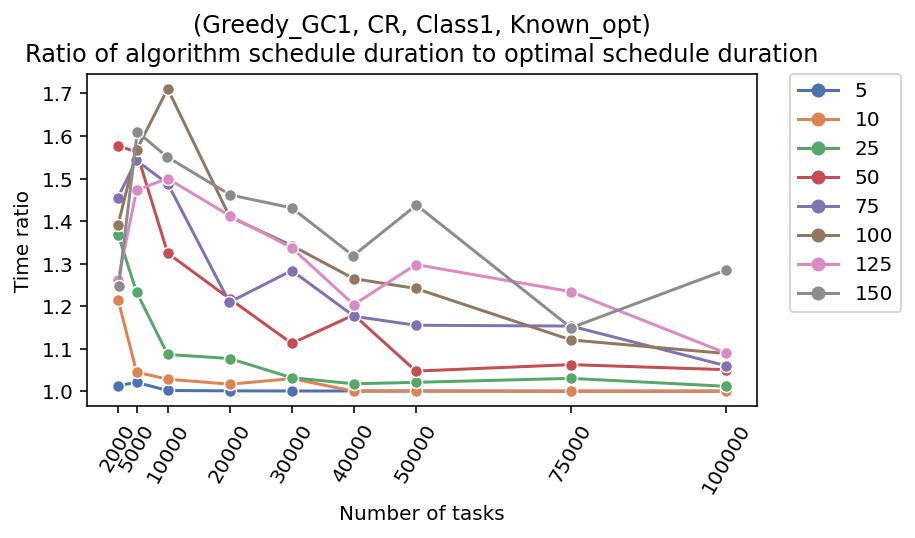
\includegraphics[width=\textwidth]{imgs/ideal_1/CR/gr_amalgamated.png}
            \caption{Жадный алгоритм с выбором по числу потомков}
        \end{subfigure}
        \begin{subfigure}{0.49\textwidth}
            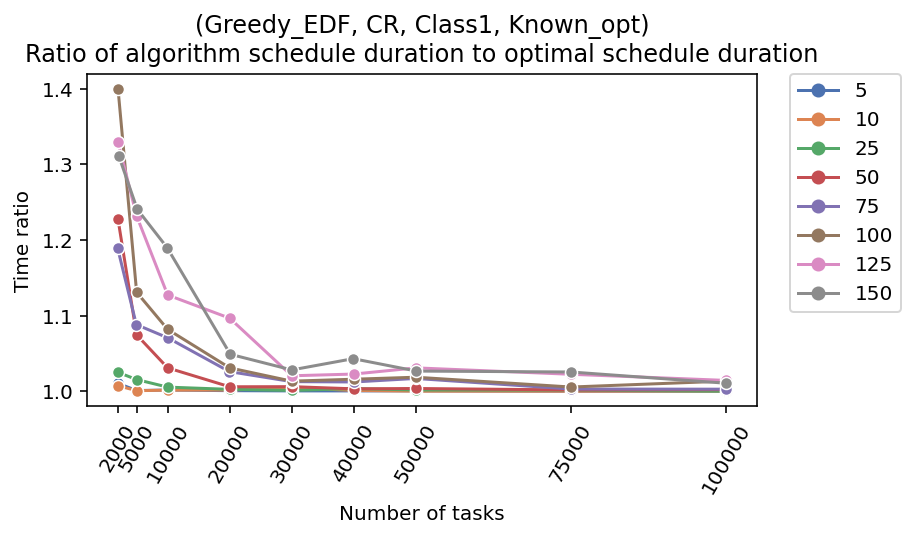
\includegraphics[width=\textwidth]{imgs/ideal_1/CR_EDF/gr_amalgamated.png}
            \caption{Жадный алгоритм с фиктивными директивными сроками}
        \end{subfigure}
        \caption{Качество решений алгоритмов на данных с известным оптимумом,\\ постановка с дополнительным ограничением на межпроцессорные передачи}
    \end{figure}
\end{frame}

\begin{frame}
    \frametitle{Точность полученного расписания. NO}
    \begin{figure}
        \begin{subfigure}{0.49\textwidth}
            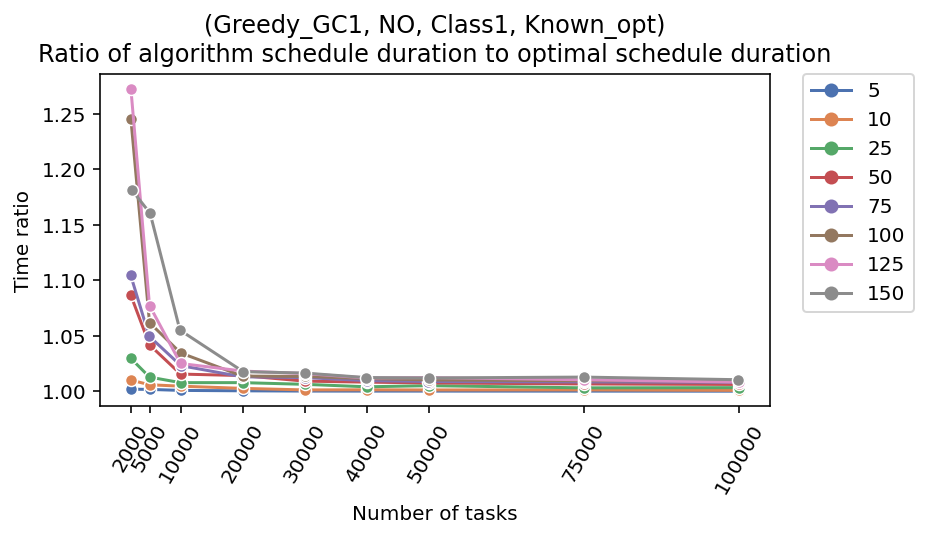
\includegraphics[width=\textwidth]{imgs/ideal_1/NO/gr_amalgamated.png}
            \caption{Жадный алгоритм с выбором по числу потомков}
        \end{subfigure}
        \begin{subfigure}{0.49\textwidth}
            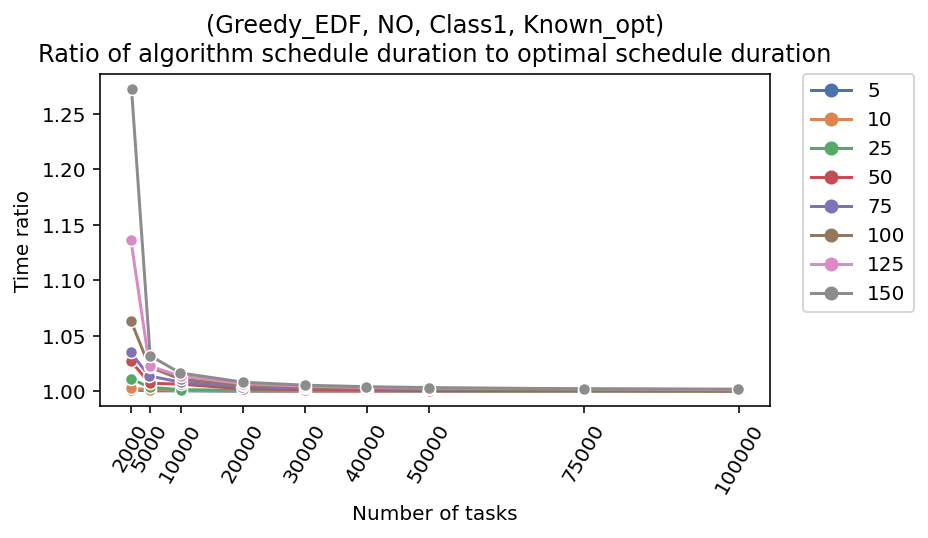
\includegraphics[width=\textwidth]{imgs/ideal_1/NO_EDF/gr_amalgamated.png}
            \caption{Жадный алгоритм с фиктивными директивными сроками}
        \end{subfigure}
        \caption{Качество решений алгоритмов на данных с известным оптимумом,\\ постановка без дополнительных ограничений}
    \end{figure}
\end{frame}



\section{Полученные рещультаты}
\begin{frame}
    \frametitle{Текущие результаты}
    \begin{enumerate}
        \item Проведен аналитический обзор алгоритмов построения списочных расписаний с целью выявления алгоритмов, которые возможно модифицировать под поставленную задачу и имеют хорошую возможность масштабирования, по результатам которого были выбраны жадные алгороитма.
        \item Разработаны и ревлизованы алгоритмы, основанные на различных жадных критериях.
        \item Проведено исследование свойств алгоритма, которое показало низкую вычислительную сложность и среднее отклонение от оптимума в 30\% для жадного алгоритма с выбором по числу потомков и до 5-10\% для жадного алгоритма с фиктивными директивными сроками. 
    \end{enumerate}
\end{frame}

\end{document}